\documentclass{article}
\usepackage[margin=1in]{geometry}
\usepackage{amsmath, amssymb, amsthm}
\usepackage{enumitem}
\usepackage{tikz}
\usetikzlibrary{calc, matrix, positioning}

\newtheorem*{lemma}{Lemma}
\newtheorem*{proposition}{Proposition}

%Cases Environment
\newlist{Cases}{enumerate}{3}
\setlist[Cases]{leftmargin = .25in, label = {Case \arabic*.}, topsep = 0.01in, itemsep = 0.04in, itemindent = .5in, parsep = 0in}

%Formatting and Spacing
\setitemize[1]{noitemsep, parsep = 5pt, topsep = 5pt}
\setenumerate[1]{label = (\alph*), parsep = 1pt, topsep = 5pt}
\setlength\parindent{0pt}
\linespread{1.1}

%Custom Title Fields
\newcommand{\lectTitle}{Lecture 11 Notes}
\newcommand{\lectTime}{February 16, 2022}
\newcommand{\lectClass}{Honors Discrete Mathematics}
\newcommand{\lectClassInstructor}{Gerandy Brito}
\newcommand{\lectSection}{Spring 2022}
\newcommand{\lectAuthorName}{Sarthak Mohanty}

%Headers and Footers
\usepackage{fancyhdr}
\usepackage{extramarks}
\pagestyle{fancy}
\lhead{\lectTime}
\chead{\lectClass \ (\lectClassInstructor)}
\rhead{\lectTitle}
\cfoot{\thepage}
\renewcommand\headrulewidth{0.4pt}
\renewcommand\footrulewidth{0.4pt}

\title{
    \vspace{2in}
    \textbf{\lectClass:\\ \lectTitle}\\
    \vspace{0.1in}\large{\textit{\lectClassInstructor\ \lectSection}}
    \vspace{3in}
    \author{\textbf{\lectAuthorName}}
    \date{}
}

\begin{document}

\maketitle
\pagebreak

\section*{Ordering Relations}
Recall that a relation $\preceq$ on a set $A$ is a \textit{partial order} if it is reflexive, antisymmetric, and transitive. In this case, the pair $(A, \preceq)$ is called a \textit{partially ordered set}, or \textit{poset}.

\subsection*{Examples}

\begin{itemize}
    \item $(\mathbb{N}, \le)$
    \item $(\mathbb{N}, \mid)$, where $a \mid b$ means that $a$ divides $b$
    \item $([n], \le)$, where $[n] = \{1, 2, \dots, n\}$
    \item $([n], \mid)$
    \item $(\mathcal{P}(S), \subseteq)$
    \item $(\prod_{i = 1}^{n} A_i, \le)$ with coordinatewise order, when each $A_i$ is ordered
\end{itemize}

\textbf{Definition.} A poset $(A, \preceq)$ is \textit{totally ordered} if every pair of elements is comparable: for all $a, b \in A$, either $a \preceq b$ or $b \preceq a$. It is \textit{well ordered} if every nonempty subset of $A$ has a least element.

\textbf{Definition.} Let $(A, \preceq)$ be a poset. An element $a \in A$ is called \textit{minimal} if there is no element $x \in A$ with $x \preceq a$ and $x \ne a$. Similarly, $a$ is called \textit{maximal} if there is no element $x \in A$ with $a \preceq x$ and $x \ne a$.

\textbf{Example.} Consider the poset $([6], \mid)$. Its Hasse diagram is
\begin{center}
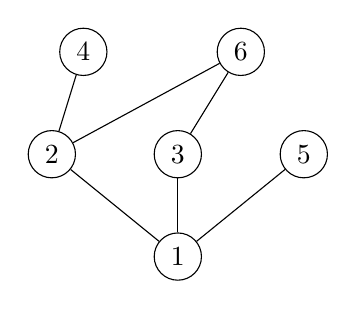
\begin{tikzpicture}[hasse node/.style={draw, circle, inner sep=1pt, minimum size=6mm}]
    \node[hasse node] (one) at (0,0) {$1$};
    \node[hasse node] (two) at (-1.6,1.3) {$2$};
    \node[hasse node] (three) at (0,1.3) {$3$};
    \node[hasse node] (five) at (1.6,1.3) {$5$};
    \node[hasse node] (four) at (-1.2,2.6) {$4$};
    \node[hasse node] (six) at (0.8,2.6) {$6$};

    \draw (one) -- (two);
    \draw (one) -- (three);
    \draw (one) -- (five);
    \draw (two) -- (four);
    \draw (two) -- (six);
    \draw (three) -- (six);
\end{tikzpicture}
\end{center}
The maximal elements are $4$, $5$, and $6$.

\begin{lemma}
If $(A, \preceq)$ is a finite poset, then $A$ has at least one minimal element. If $(A, \preceq)$ is totally ordered, then this minimal element is unique.
\end{lemma}

\begin{proof}
Pick any $a \in A$. If $a$ is minimal, we are done. Otherwise, there exists some $a_1 \ne a$ such that $a_1 \preceq a$. If $a_1$ is not minimal, repeat the process. Since $A$ is finite, this process must eventually stop, and it stops exactly at a minimal element.

Now suppose $(A, \preceq)$ is totally ordered and let $m_1$ and $m_2$ be minimal elements. Since the order is total, either $m_1 \preceq m_2$ or $m_2 \preceq m_1$. By minimality, this forces $m_1 = m_2$.
\end{proof}

\textbf{Example.} In $(\mathcal{P}(\{1, 2, 3, 4\}), \subseteq)$, the Hasse diagram is the Boolean lattice:
\begin{center}
{\scriptsize
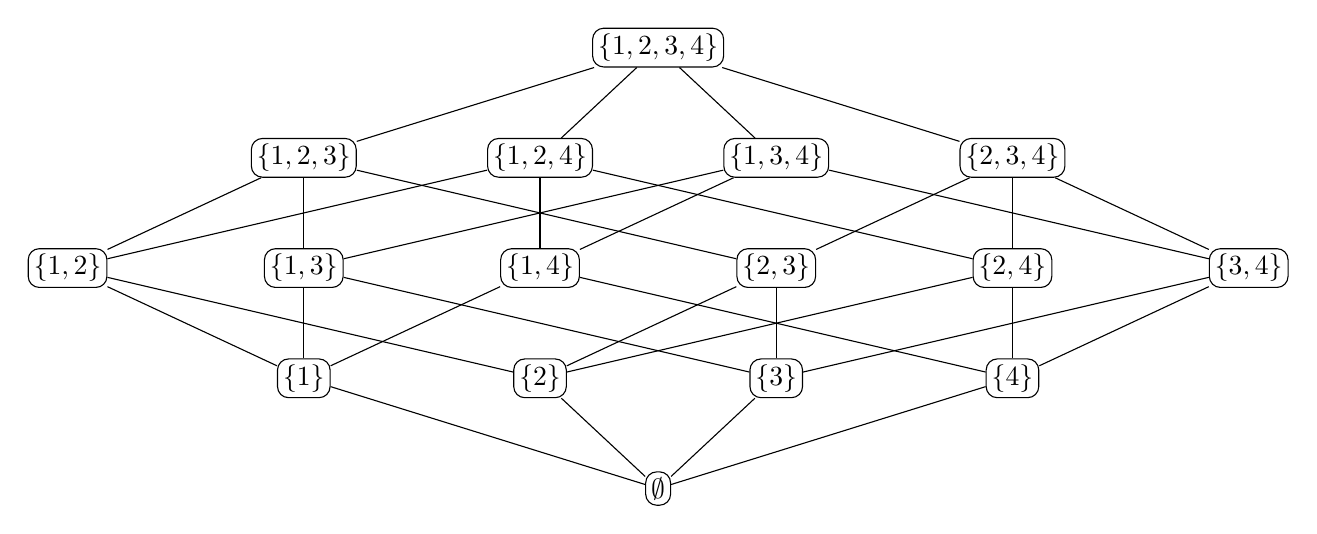
\begin{tikzpicture}[subset node/.style={draw, rounded corners, inner sep=2pt}]
    \node[subset node] (empty) at (0,0) {$\emptyset$};

    \node[subset node] (one) at (-4.5,1.4) {$\{1\}$};
    \node[subset node] (two) at (-1.5,1.4) {$\{2\}$};
    \node[subset node] (three) at (1.5,1.4) {$\{3\}$};
    \node[subset node] (four) at (4.5,1.4) {$\{4\}$};

    \node[subset node] (onetwo) at (-7.5,2.8) {$\{1,2\}$};
    \node[subset node] (onethree) at (-4.5,2.8) {$\{1,3\}$};
    \node[subset node] (onefour) at (-1.5,2.8) {$\{1,4\}$};
    \node[subset node] (twothree) at (1.5,2.8) {$\{2,3\}$};
    \node[subset node] (twofour) at (4.5,2.8) {$\{2,4\}$};
    \node[subset node] (threefour) at (7.5,2.8) {$\{3,4\}$};

    \node[subset node] (onetwothree) at (-4.5,4.2) {$\{1,2,3\}$};
    \node[subset node] (onetwofour) at (-1.5,4.2) {$\{1,2,4\}$};
    \node[subset node] (onethreefour) at (1.5,4.2) {$\{1,3,4\}$};
    \node[subset node] (twothreefour) at (4.5,4.2) {$\{2,3,4\}$};

    \node[subset node] (all) at (0,5.6) {$\{1,2,3,4\}$};

    \draw (empty) -- (one);
    \draw (empty) -- (two);
    \draw (empty) -- (three);
    \draw (empty) -- (four);

    \draw (one) -- (onetwo);
    \draw (one) -- (onethree);
    \draw (one) -- (onefour);
    \draw (two) -- (onetwo);
    \draw (two) -- (twothree);
    \draw (two) -- (twofour);
    \draw (three) -- (onethree);
    \draw (three) -- (twothree);
    \draw (three) -- (threefour);
    \draw (four) -- (onefour);
    \draw (four) -- (twofour);
    \draw (four) -- (threefour);

    \draw (onetwo) -- (onetwothree);
    \draw (onetwo) -- (onetwofour);
    \draw (onethree) -- (onetwothree);
    \draw (onethree) -- (onethreefour);
    \draw (onefour) -- (onetwofour);
    \draw (onefour) -- (onethreefour);
    \draw (twothree) -- (onetwothree);
    \draw (twothree) -- (twothreefour);
    \draw (twofour) -- (onetwofour);
    \draw (twofour) -- (twothreefour);
    \draw (threefour) -- (onethreefour);
    \draw (threefour) -- (twothreefour);

    \draw (onetwothree) -- (all);
    \draw (onetwofour) -- (all);
    \draw (onethreefour) -- (all);
    \draw (twothreefour) -- (all);
\end{tikzpicture}
}
\end{center}
The minimal element is $\emptyset$, and the maximal element is $\{1,2,3,4\}$.

\subsection*{Least Upper Bounds}

\textbf{Definition.} Given a poset $(A, \preceq)$ and a subset $S \subseteq A$, an \textit{upper bound} for $S$ is an element $u \in A$ such that $s \preceq u$ for all $s \in S$. A \textit{least upper bound}, written $\operatorname{lub}(S)$, is an upper bound $y$ such that $y \preceq x$ for every upper bound $x$ of $S$.

Analogously, a \textit{greatest lower bound}, written $\operatorname{glb}(S)$, is a lower bound $y$ such that $x \preceq y$ for every lower bound $x$ of $S$.

\textbf{Example.} Consider the poset $(A, \mid)$, where
\[
A = \{1,2,3,4,5,6,7,8,9,10\}.
\]
Its Hasse diagram is
\begin{center}
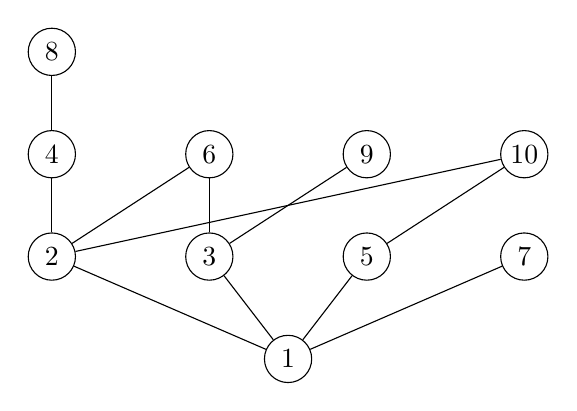
\begin{tikzpicture}[hasse node/.style={draw, circle, inner sep=1pt, minimum size=6mm}]
    \node[hasse node] (one) at (0,0) {$1$};

    \node[hasse node] (two) at (-3,1.3) {$2$};
    \node[hasse node] (three) at (-1,1.3) {$3$};
    \node[hasse node] (five) at (1,1.3) {$5$};
    \node[hasse node] (seven) at (3,1.3) {$7$};

    \node[hasse node] (four) at (-3,2.6) {$4$};
    \node[hasse node] (six) at (-1,2.6) {$6$};
    \node[hasse node] (nine) at (1,2.6) {$9$};
    \node[hasse node] (ten) at (3,2.6) {$10$};

    \node[hasse node] (eight) at (-3,3.9) {$8$};

    \draw (one) -- (two);
    \draw (one) -- (three);
    \draw (one) -- (five);
    \draw (one) -- (seven);
    \draw (two) -- (four);
    \draw (two) -- (six);
    \draw (two) -- (ten);
    \draw (three) -- (six);
    \draw (three) -- (nine);
    \draw (five) -- (ten);
    \draw (four) -- (eight);
\end{tikzpicture}
\end{center}
Then
\[
\operatorname{lub}(\{1,2,3\}) = 6,\qquad \operatorname{lub}(\{1,2,4\}) = 4.
\]
The set $\{3,5,7\}$ has no least upper bound in this poset.

\begin{lemma}
If a least upper bound exists, then it is unique.
\end{lemma}

\begin{proof}
Let $x$ and $y$ both be least upper bounds for $S$. Since $x$ is a least upper bound and $y$ is an upper bound, $x \preceq y$. Since $y$ is a least upper bound and $x$ is an upper bound, $y \preceq x$. By antisymmetry, $x = y$.
\end{proof}

\textbf{Definition.} A poset is called a \textit{lattice} if every pair of elements has both a least upper bound and a greatest lower bound.

\textbf{Example.} The poset $(\mathbb{N}, \mid)$ is a lattice. For $a, b \in \mathbb{N}$,
\[
\operatorname{lub}(\{a,b\}) = \operatorname{lcm}(a,b)
\qquad\text{and}\qquad
\operatorname{glb}(\{a,b\}) = \gcd(a,b).
\]
Indeed, if $d = \gcd(a,b)$ and $c = \operatorname{lcm}(a,b)$, then
\[
d \mid a,\quad d \mid b,\quad a \mid c,\quad b \mid c.
\]
Moreover, $d$ is the greatest common divisor and $c$ is the least common multiple, so they have exactly the required universal properties.

\subsection*{Topological Sorting}

Topological sorting is useful when a poset represents prerequisites or dependencies. For example, let
\[
A = \{\mathrm{CS1}, \mathrm{CS2}, \dots, \mathrm{CS}n\},
\]
and define $a \preceq b$ if course $a$ must be taken before course $b$. One possible Hasse diagram is
\begin{center}
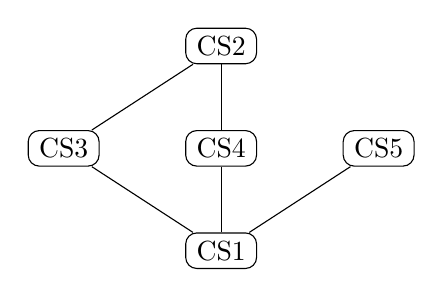
\begin{tikzpicture}[course node/.style={draw, rounded corners, inner sep=3pt, minimum width=9mm}]
    \node[course node] (cs1) at (0,0) {$\mathrm{CS1}$};
    \node[course node] (cs3) at (-2,1.3) {$\mathrm{CS3}$};
    \node[course node] (cs4) at (0,1.3) {$\mathrm{CS4}$};
    \node[course node] (cs5) at (2,1.3) {$\mathrm{CS5}$};
    \node[course node] (cs2) at (0,2.6) {$\mathrm{CS2}$};

    \draw (cs1) -- (cs3);
    \draw (cs1) -- (cs4);
    \draw (cs1) -- (cs5);
    \draw (cs3) -- (cs2);
    \draw (cs4) -- (cs2);
\end{tikzpicture}
\end{center}

\textbf{Definition.} Given a finite poset $(A, \preceq)$, a \textit{topological sorting} of $A$ is an enumeration
\[
a_1, a_2, \dots, a_n
\]
of the elements of $A$ such that if $a_i \preceq a_j$, then $i \le j$.

Every finite poset has a topological sorting: choose a minimal element, remove it, and repeat this process on the remaining poset until no elements are left.

\textbf{Example.} Consider $(\{1,2,4,5,10,20\}, \mid)$. Its Hasse diagram is
\begin{center}
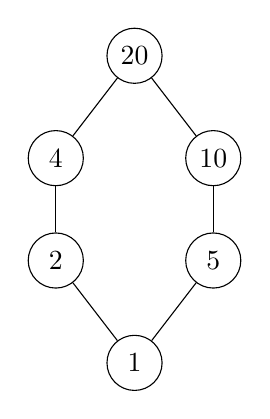
\begin{tikzpicture}[hasse node/.style={draw, circle, inner sep=1pt, minimum size=7mm}]
    \node[hasse node] (one) at (0,0) {$1$};
    \node[hasse node] (two) at (-1,1.3) {$2$};
    \node[hasse node] (five) at (1,1.3) {$5$};
    \node[hasse node] (four) at (-1,2.6) {$4$};
    \node[hasse node] (ten) at (1,2.6) {$10$};
    \node[hasse node] (twenty) at (0,3.9) {$20$};

    \draw (one) -- (two);
    \draw (one) -- (five);
    \draw (two) -- (four);
    \draw (five) -- (ten);
    \draw (four) -- (twenty);
    \draw (ten) -- (twenty);
\end{tikzpicture}
\end{center}
A topological sorting is
\[
1, 5, 2, 10, 4, 20.
\]
Another valid topological sorting is
\[
1, 2, 5, 4, 10, 20.
\]
For a totally ordered finite set, there is exactly one topological sorting.

\begin{proposition}
Let $(A, \preceq)$ be a finite poset. If $A$ has a unique topological sorting, then $A$ is totally ordered.
\end{proposition}

\begin{proof}
Let
\[
a_1, a_2, \dots, a_n
\]
be the unique topological sorting of $A$. We claim that each consecutive pair $a_i, a_{i+1}$ is comparable. Suppose not. Then $a_i$ and $a_{i+1}$ are incomparable, so switching their positions still gives a valid topological sorting:
\[
a_1, a_2, \dots, a_{i+1}, a_i, \dots, a_n.
\]
This contradicts uniqueness.

Therefore $a_i$ and $a_{i+1}$ are comparable for every $i$. Since the original order is topological, we must have $a_i \preceq a_{i+1}$ for every $i$. By transitivity, $a_i \preceq a_j$ whenever $i \le j$. Thus every pair of elements in $A$ is comparable, so $A$ is totally ordered.
\end{proof}
\end{document}
